\documentclass{mistcoursedoc}
\usepackage[french]{babel}
\usepackage[utf8]{inputenc}
\usepackage{paralist}


\course{INF3995: Projet de conception d’un\\ système informatique}
\term{Hiver}
\termyears{2021} 
\doctype{Réponse à l’appel d’offres}

% Numéro équipe
\newcommand{\equipe}{203}
\newcolumntype{M}[1]{>{\raggedright}m{#1}}
\author{Équipe \equipe}

\begin{document}

\maketitle
\vspace{2cm}
\begin{center}

  {\Huge\bf Système aérien minimal pour exploration\\[3em]}

  \Large Proposition répondant à l’appel d’offres  n°H2021-INF3995 du département GIGL\\[3em]


  Équipe No. \equipe\\[3em]

  Bal, Samba Bousso\\[1em]
  Chritin, Mathurin\\[1em]
  Grootenboer, Hubert\\[1em]
  Maghni, Issam Eddine\\[1em]
  Sangam, Eya-Tom Augustin\\[1em]

  \vfill

\end{center}

\newpage
{
  \renewcommand{\contentsname}{Table des matières}
  \hypersetup{hidelinks}
  \setcounter{secnumdepth}{3}
  \setcounter{tocdepth}{3}
  \tableofcontents
}
\newpage

\section*{Introduction}
La robotique a fait partie de notre travail depuis maintenant 2 ans (notamment pendant projet nommé « Projet Initial de système embarqué ») réalisé il y a un an et demi. Cet appel d'offre sur un système aérien minimal d'exploration figurait donc naturellement au sommet de la liste des offres que nous souhaitons décrocher. Nous sommes une équipe de 5 personnes fondamentalement motivés par les systèmes embarqués et nous serions heureux de pouvoir vous faire profiter de notre expertise et de notre engouement pour ce projet. Nous sommes convaincus que nous arriverons à satisfaire vos exigences de la meilleure des manières, en vous offrant de la flexibilité et en restant à l'écoute de vos remarques tout au long de ce projet.

\section{Vue d’ensemble du projet}

\subsection{But du projet, portée et objectifs}

\par L'objectif principal de ce projet est de créer un système informatique de gestion de drones.
Ledit système est un ensemble de logiciels qui permettra à un essaim composé d’un nombre arbitraire de drones (quadricoptères) miniatures (<250grammes) d’explorer une pièce d’un bâtiment de moyenne dimension à l'aide de capteurs lasers et de reporter ces informations à une interface opérateur basée sur le Web. 
Un opérateur, en utilisant cette interface, doit être en mesure de démarrer le système, l’arrêter, et mettre à jour le logiciel de bord des drones. Le système à concevoir est composé de deux parties (voir Figure \ref{fig:systeme}).

\begin{figure}[h!]
  \centering\includegraphics[width=0.7\textwidth]{systeme.png}
  \caption{Système à concevoir}
  \label{fig:systeme}
\end{figure}

\begin{itemize}
    \item Station au sol: il s’agit d’un ordinateur avec une interface Web qui peut communiquer avec les drones à travers un canal de communication à 2.4 GHz. Nous supposons qu’au moins un robot de l’essaim est toujours en communication avec la station au sol;
    \item Partie embarquée: il s’agit des drones et du logiciel qui roule sur leur micro-contrôleur de bord. Les drones communiquent entre eux et avec la station à travers un canal de communication à 2.4GHz. 
\end{itemize}

L’opérateur utilise un navigateur Web pour contrôler le système et visualiser les données générées par les drones. Le produit complet sera livré accompagné d’une démonstration vidéo.

\par Un tel système se révélera très utile durant les explorations sur Mars, encore peu connue de tous.
Nous imaginons une situation dans laquelle un robot plus complexe,
plus lent et limité dans sa capacité de mouvement, se fera diriger par une colonie de drones qui
lui indiquera les endroits les plus intéressants à explorer.

\subsection{Hypothèses et contraintes}

\subsubsection{Hypothèses sur l'utilisation du système}

\begin{itemize}

  \item \textbf{Utilisation du système} :\\
        Le système conçu sera utilisé uniquement à des fins d'explorations et non d'espionnage.
        Selon le milieu exploré, l'utilisateur du système se devra d'obtenir les autorisations nécessaires conformément au lois régissant le lieu d’utilisation.
  \item \textbf{Sécurité} :\\
        L'opérateur du système devra être âgé d'au moins 16 ans et devra se munir de lunettes de sécurité durant toute
        interaction avec le drone.
  \item \textbf{Milieu exploré} :\\
        Le milieu exploré devra se trouver dans des conditions météorologiques convenables.
        Idéalement, une pièce fermée à température ambiante.

\end{itemize}

\subsubsection{Contraintes matérielles}
\begin{itemize}

  \item \textbf{Les drones} : \\
        L’opérateur du système devra posséder au moins deux kits Bitcraze Crazyfly 2.0 STEM Bundle.
        Uniquement le « Flow deck » et le « Ranger Deck » fournis dans les kits devront être installés sur les drones.

  \item \textbf{La station au sol} : \\
        L’ordinateur de la station de contrôle devra être muni d’un système d’exploitation
        Linux, virtualisé ou non, possédant au minimum 4 Gio de mémoire vive.
        Un fureteur à jour et un terminal doivent être présent sur l’ordinateur.

  \item \textbf{Communication avec la station au sol} : \\
        Le seul moyen de communication entre la station au sol et les drones doit être
        l’antenne Bitcraze CrazyradioPA connectée à la station au sol.

\end{itemize}

\subsubsection{Contraintes fonctionnelles}
Le système devrait être en mesure de répondre au contraintes ci-dessous :

\begin{itemize}
  \item \textbf{Commandes supportées} :\\
        Les commandes sont des instructions envoyées depuis l'interface de contrôle
        aux drones. Trois commandes devraient pour être supportées par les drones :
        \begin{itemize}
          \item Lancer la mission : \\
                Une fois la commande de départ reçue, les drones doivent être capables de parcourir le périmètre
                d’une pièce d’au maximum 100 $m^2$ en absence d’autres commandes de la station au sol. \\
                Durant cette opération, les drones doivent éviter les obstacles sur leur chemin, incluant les autres drones.\\
                L’algorithme d’exploration de l’environnement n’a pas de contraintes.
                Cela peut être une séquence de mouvements aléatoires. Cependant l'exploration doit se faire
                de façon à pouvoir générer une carte du milieu exploré.\\
                Les drones ne doivent pas décoller avec un niveau de batterie inférieur à 30\%.
          \item Fin de mission : \\
                Cette commande permet d'arrêter l'exploration. Après cette commande, les drones se mettre en
                position stable en attendant une autre commande de la station au sol.
          \item Retour à la base : \\
                Le retour à la base doit rapprocher les drones à moins de 1m de la station à terre.
                Le retour à la base et l’atterrissage doivent s’enclencher automatiquement dès que le niveau
                de batterie passe en dessous de 30\%.
                Mise à jour logicielle : \\
                L’interface doit permettre la mise à jour du logiciel interne des drones seulement s’ils se trouvent au sol. La mise à jour doit être implémentée comme l’envoi d’un paquet binaire en utilisant l’API de BitCraze.
        \end{itemize}
        \par
        En dehors de ces commandes, le robot devrait toujours se mettre dans un état cohérent si un accident survient.
        La Figure \ref{fig:fsm} montre un aperçu des différents états du robot suivant les commandes reçues.
        \begin{figure}[h!]
          \centering\includegraphics[width=0.9\textwidth]{fsm.png}
          \caption{Diagramme montrant les différents états et interactions possibles avec un drone}
          \label{fig:fsm}
        \end{figure}

        Les données suivantes seront mise à jour avec une fréquence minimale de 1Hz:
        \begin{enumerate}
          \item Nombre des drones
          \item État des drones (en attente, en mission, accidenté)
          \item Vitesse courante des drones
          \item Niveau de batterie des drones
          \item Carte générée durant l’exploration
          \item Position des drones
          \item Éditeur pour le code du drone
        \end{enumerate}

    \item \textbf{// TODO: Comprendre ceci} :\\
        L’intégration des mesures des différents drones est faite par la station au sol en supposant
        que les positions et orientations initiales des drones sont connues ou [OPTIONNEL] en résolvant un
        problème d’optimisation permettant d’inférer la carte la plus plausible selon
        les données recueillies(Maximum Likelihood Estimation).

\end{itemize}

\subsubsection{Contraintes de temps}
La charge requise en termes d’heures pour la livraison du projet est de 630 heures-personnes.
Plus de détails sont disponibles à la section \ref{calendrier}.

Un version finale du projet sera livrée pour le lundi 19 avril 2021 en avant-midi.

\subsection{Biens livrables du projet}
\textit{Énumérer les artefacts qui devront être créés durant le projet avec leurs dates prévues de publication.}


Notre application sera composée de trois briques : un tableau de bord accessible par l'opérateur, un serveur maître + base de données faisant l'intermédiaire avec le tableau de bord et les drones, et le micrologiciel embarqué sur les drones.
\begin{itemize}
  \item \textbf{Prototype minimal} : afin de démontrer au client la maîtrise des technologies utilisées (\textit{date prévue 2021-02-15}):
        \begin{itemize}
          \item Interface web minimale avec boutons de décollage (« Take Off ») et d’atterrissage (« Land »), ainsi que le niveau de batterie, la position et la vitesse du drone en action dans le simulateur ARGoS 3.
          \item Serveur maître basique faisant l’intermédiaire entre le simulateur et l’interface web : relais les messages de mise à jour en temps réel des drones vers le client web, et transfert les commandes du client web vers les drones, le tout à l'aide d'une \emph{socket} TCP. Pas encore de concept de base de donnée.
          \item Version basique du micrologiciel : récupération des données de la batterie et de la vitesse, encodage en JSON et envoie des données vers une \emph{socket} TCP
          \item Simulateur ARGoS faisant bouger deux drones
        \end{itemize}
  \item \textbf{Prototype intermédiaire} : pour démontrer au client l'avancement du projet (\textit{date prévue 20201-03-08}) :
        \begin{itemize}
          \item Interface web avancée, fonctionnalité de retour à la base (« Return to base ») implémentés, et visualisation minimale des données captées par les drones
          \item Simulateur avec quatre drones évoluant dans un environnement généré aléatoirement en évitant les obstacles
          \item Serveur maître et micrologiciel avancés pour répondre aux besoins de la démonstration décrite par les points susmentionnés
        \end{itemize}
        % TODO move somewhere else
        % \begin{itemize}
        %   \item Interface web évoluée, avec de quoi afficher les données visualisées par le drone en temps réel sous forme de graphe.
        %   \item Serveur maître évolué, implémentant un premier modèle de base de donnée capable de stocker en temps réel des données quelconques (en attendant de pouvoir stocker les informations sur les obstacles émises par les drones).
        %   \item Micrologiciel évolué : capable de retrouver les données des capteurs de distance et de les interpréter pour faire varier l'itinéraire du drone en fonction de ces informations.
        % \end{itemize}
  \item \textbf{Démonstration finale}, mettant en jeu : ????????
        \begin{itemize}
          \item L'interface web finale avec les boutons « TakeOff » et « Return to base » comme seules commandes pour lancer et terminer la mission, et affichage de toutes les informations des drones en temps réel
          \item Le serveur maître final pour interfacer les commandes de l'interface web et traiter les données reçues des drones
          \item Le tout sous la forme d'une vidéo pour montrer le comportement des drones dans un environnement qu'il ne connaît pas
        \end{itemize}
\end{itemize}

\section{Organisation du projet}

\subsection{Structure d’organisation}

\textit{Décrire la structure d’organisation de l’équipe de projet et les différents rôles des membres.}
L’équipe est composée de 5 membres. Ils participeront au développement de la solution à tous les niveaux (client, serveur et micrologiciel), et seront en tout temps au courant de l’avancement des différents artefacts du projet. Un membre de l'équipe, M. Samba Bal, assumera le rôle du gestionnaire de projet pour organiser le développement. GitLab sera utilisé pour gérer les tâches à effectuer, les assigner aux différents membres et comptabiliser le temps passé sur chacune d’elles.

\subsection{Entente contractuelle}

\textit{Décrire le type d’entente contractuelle proposée pour projet et les raisons de ce choix}

Un contrat de livraison clef en main serait adéquat pour ce projet. En effet, le contracteur a une liste des requis complète et suffisamment précise pour ne pas avoir à la modifier grandement au cours du projet.
Grâce à cela, on peut prévoir le temps nécessaire pour réaliser le projet et ainsi prévoir un coût fixe pour la réalisation du produit. Le détail de l'estimation des coûts pour ce projet est donné à la section \ref{coûts}

\section{Solution proposée}

\subsection{Architecture logicielle générale}

\textit{Un diagramme qui résume l’architecture. Un texte qui décrit et justifie les choix. Inspiration: \og L’ingénieur a parfois un peu peur de réaliser des choses parce que les moyens sont maintenant considérablement sophistiqués. On oublie que seulement prendre un papier et un crayon, décrire les choses, faire une esquisse, cela peut être aussi valable qu’un dessin d’ordinateur.}

\begin{figure}[h!]
  \centering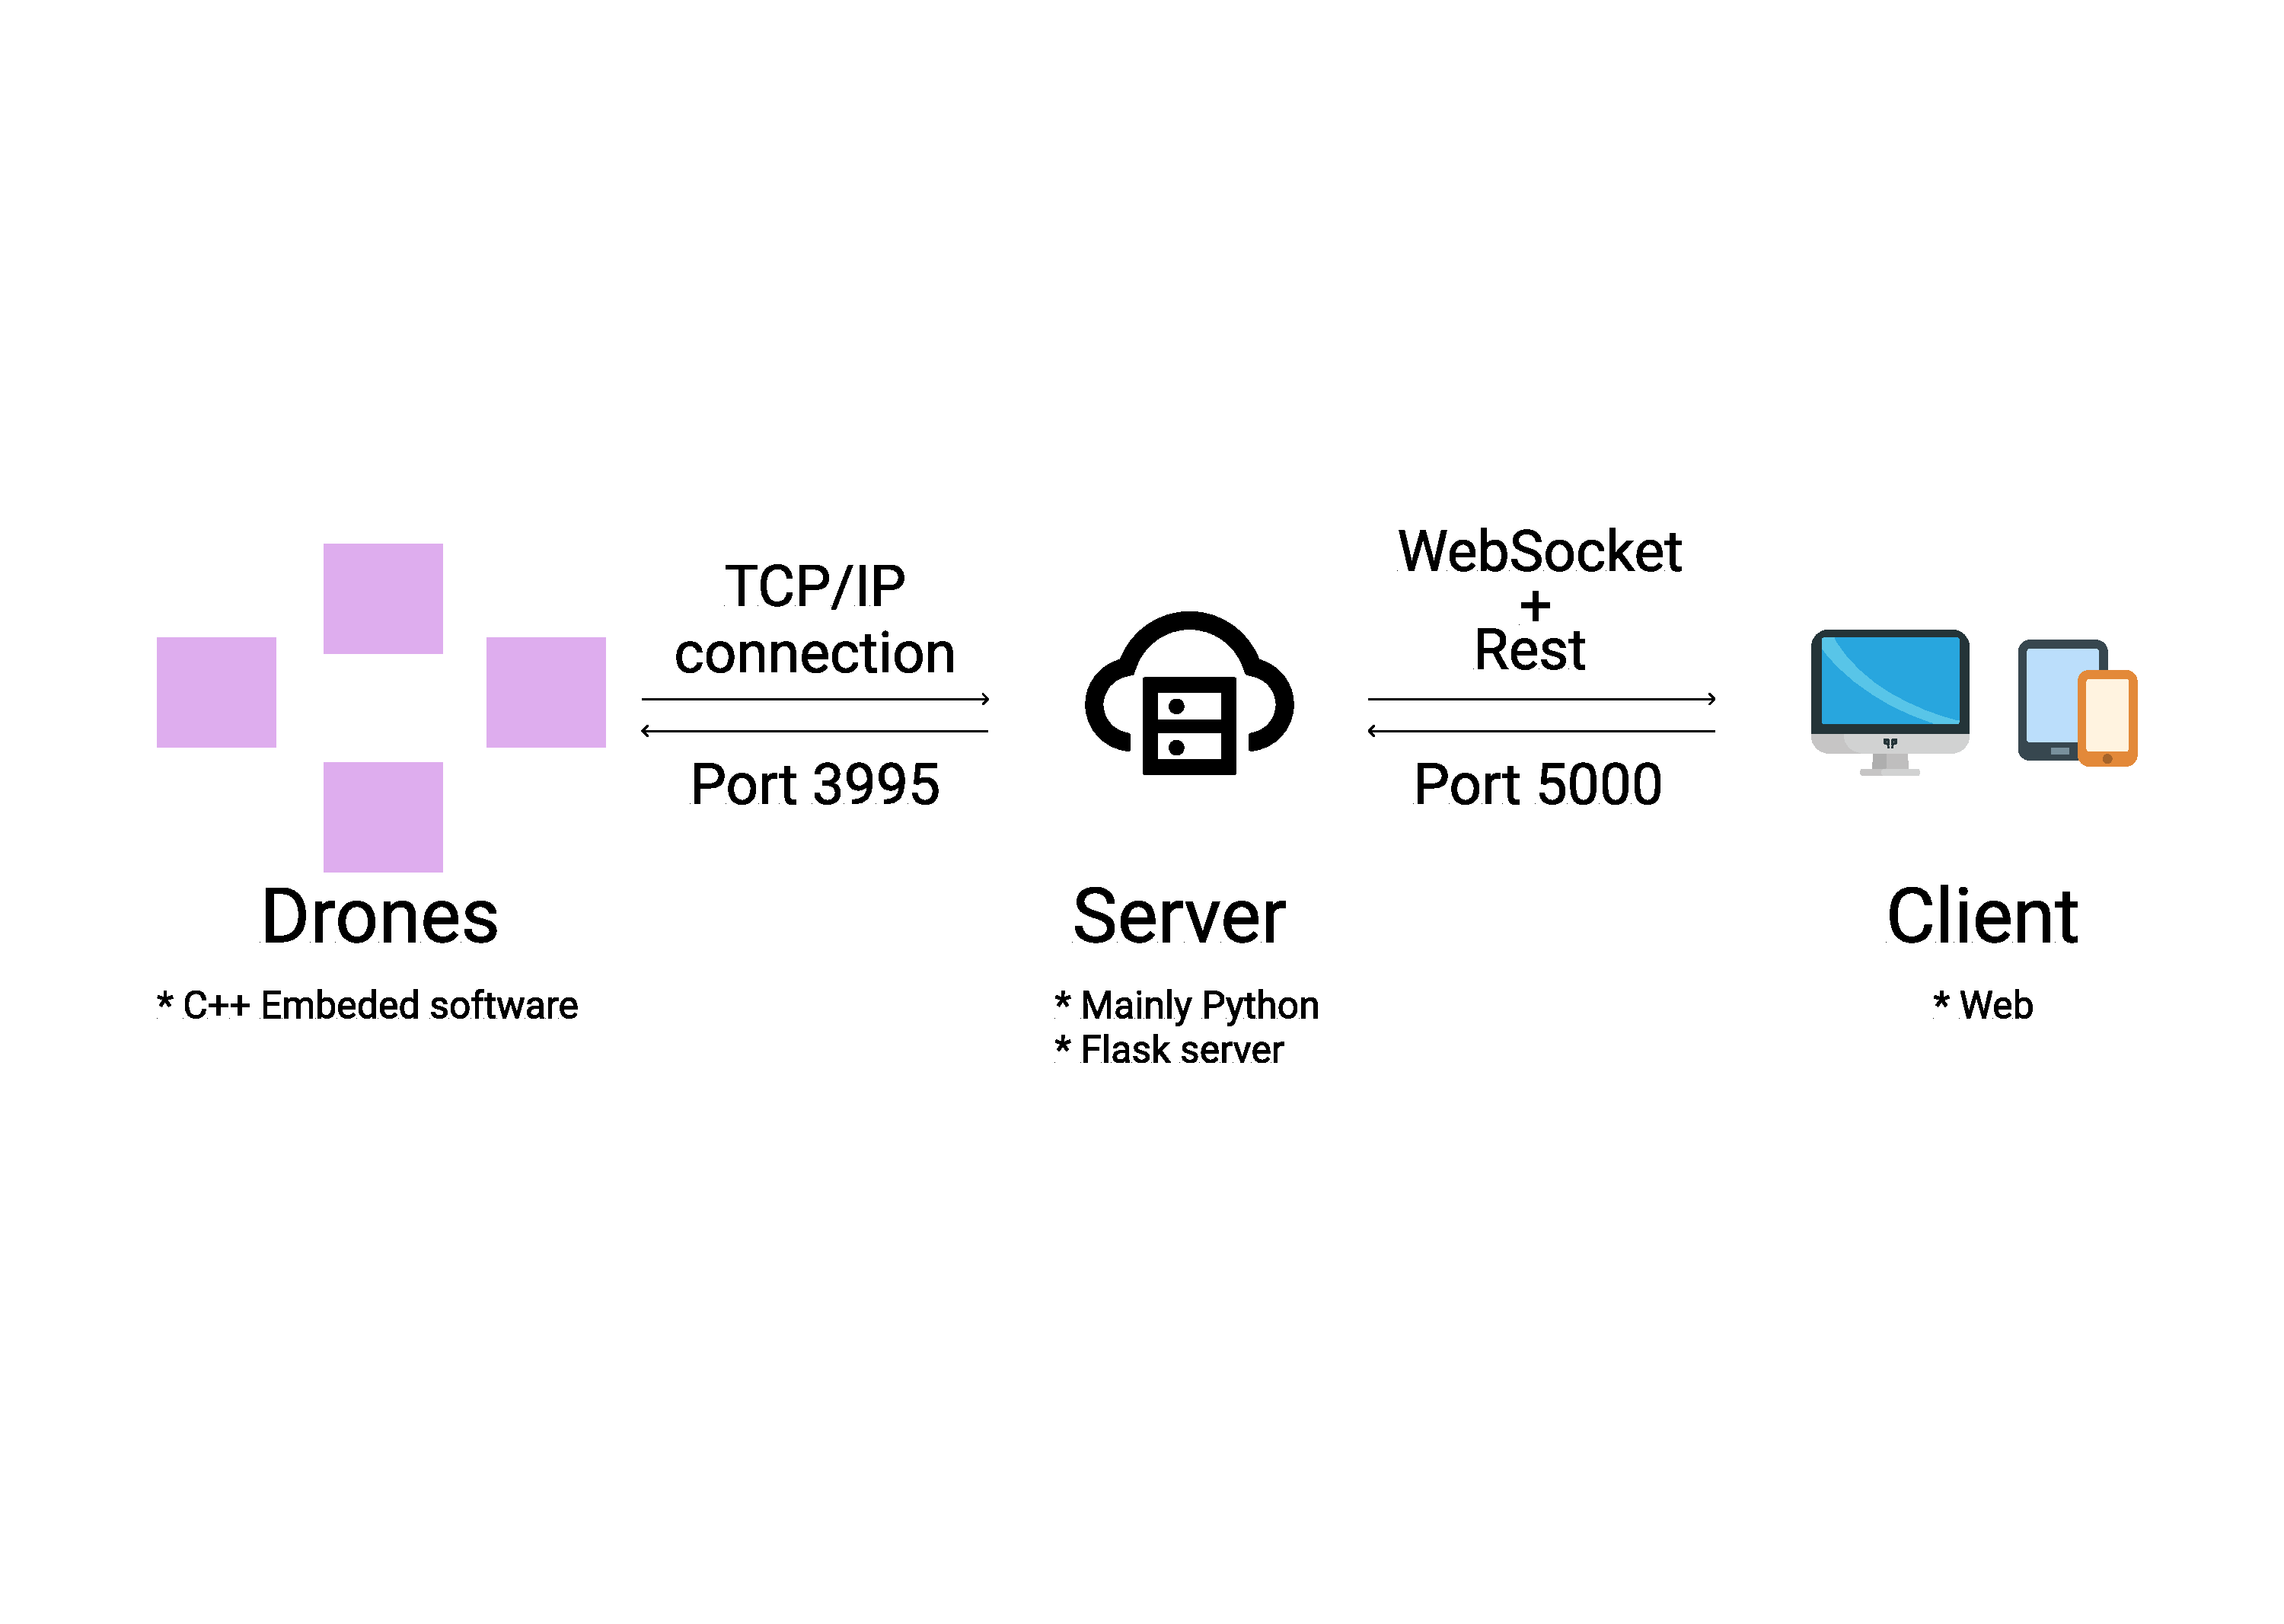
\includegraphics[width=0.9\textwidth]{architecture-globale.png}
  \caption{Architecture globale de la solution}
\end{figure}

\par La solution retenue fait état de trois entités :
\begin{itemize}
  \item Un client web : Il s'agit d’une application web utilisée par un opérateur. Il permet ainsi les interactions avec les drones
  \item Un serveur maître : Il s’agit d’un serveur centrale qui joue le rôle d'intermédiaire entre le client et les drones. Du201’une part il transmettra les commandes du client aux drones. D'autre part, il remettra au client les résultats et informations venant des différents drones.
  \item Les drones : Un ou plusieurs drones qui communiquent entre eux mais également avec le serveur central (couple client-serveur). Ils effectuent les activités d'explorations.
\end{itemize}

\par Les requis nous demandent deux modules, à savoir, une station au sol qui est un ordinateur disposant d’une interface web et d’une partie embarquée pour les drones. Nous avons par la suite subdivisé la station au sol en deux éléments qui sont le client et le serveur.

\subsection{Architecture du logiciel embarqué}
\textit{Un diagramme qui résume l architecture.  Un texte qui décrit et justifie les choix.}

Compte tenu de la situation, le simulateur ARGoS sera beaucoup utilisé pour tester le fonctionnement de notre application. Ce simulateur est fourni avec un certain nombre de fonctionnalités déjà implémentées, mais pour simuler réellement le comportement du drone dans la vie réelle, il sera nécessaire de le modifier et d'ajouter certaines couches d'abstraction que nous allons tenter d'implémenter de la manière suivante :

\begin{figure}[h!]
    \centering
    \includegraphics[width=0.9\textwidth]{firmware-architecture.png}
    \caption{Architecture du logiciel embarqué}
\end{figure}

L'objectif ici est de rassembler le plus possible la logique de notre application d'une manière à ce qu'en changeant simplement le \textttt{\#include} de la librairie utilisée, nous puissions \textit{switcher} du simulateur au drone réel et inversement. Par exemple, le simulateur communique actuellement avec le serveur maître à l'aide d'une socket TCP, mais le vrai drone utilisera la classe \texttt{AppChannel}. Nous allons donc ajouter une couche d'abstraction qui s'occupera de gérer la communication avec le serveur maître peu importe le type de drone utilisé (virtuel dans le simulateur ou réel).

\newpage\subsection{Architecture logicielle de la station au sol}

\textit{Quelques blocs des principaux modules ou classes seulement.  Des diagrammes sont nécessaires.  Un texte qui décrit et justifie les choix.}

\begin{figure}[h!]
  \centering\includegraphics[width=0.9\textwidth]{architecture-serveur.pdf}
  \caption{Architecture globale du serveur maître}
\end{figure}

Le serveur maître est composé de deux serveur, un pour gérer les communications avec les drones et un autre pour gérer les communications avec les clients. Ces deux serveurs sont nécessaires puisque les drones et les client n’utilise pas le même support de communication. Les clients utilisent une \emph{WebSocket} pour interagir avec le serveur, tandis que les drones utilisent « L'ANTENNE ». Étant donné qu'il peut y avoir plusieurs clients et plusieurs drones, les serveurs doivent lancer des instance de gestionnaire de communication pour chaque connexion établie (drone\_communication\_handler et dashboard\_communication\_handler). Ces derniers sont responsables de recevoir et d’envoyer de l’information à un seul drone/client. Le serveur maître s'occupe de faire le lien entre ces deux serveur, et de sauvegarder les informations utiles dans la base de donnée.

\newpage
\section{Processus de gestion}

\subsection{Estimations des coûts du projet}\label{coûts}

\textit{Les divers frais rattachés au projet peuvent nous aider à estimer le coût global du projet.}

Les ressources humaines constituent la principale dépense du projet.
Avec quatre développeurs-analystes et un coordonnateur de projet à temps partiel,
il est nécessaire d’avoir une estimation de temps pour en déduire le coût juste.

Pour le bien de la cause, nous disposons de 11 heures de travail par semaine et par développeur et 12 heures par semaine pour le coordonnateur.
Sachant que le projet s’échelonne sur 11 semaines, nous obtenons un total de 484 heures pour les développeurs
et 132 heures pour le coordonnateur.

\begin{table}[h!]
  \centering
  \begin{tabular}{M{6.5cm} M{3.5cm} M{3.5cm} M{1.5cm}}
    \hline
    \textbf{Tâches}                      & \textbf{Coordonnateur [h]} & \textbf{Développeurs [h]} & \textbf{Total} \tabularnewline\hline
    Description des exigences du système & 10                        & 20                        & 30 \tabularnewline
    Analyse des APIs (Bitcraze)          & 15                        & 40                        & 55 \tabularnewline
    Analyse du simulateur ARGoS 3        &                           & 10                        & 10 \tabularnewline
    Analyse des services                 & 10                        & 35                        & 45 \tabularnewline
    Analyse de la base de données        &                           & 10                        & 10 \tabularnewline
    Implémentation des services          & 25                        & 110                       & 135 \tabularnewline
    Implémentation des interfaces        & 10                        & 50                        & 60 \tabularnewline
    Tests des interfaces                 & 8                         & 10                        & 18 \tabularnewline
    Tests des services                   & 8                         & 10                        & 18\tabularnewline
    Déploiement (Docker)                 & 5                         & 4                         & 9\tabularnewline
    Tests finaux                         & 6                         & 10                        & 16 \tabularnewline\hline
    Total [h]                            & 97                        & 309                       & \textbf{406h} \tabularnewline
    Total [\$]                           & 14'065                    & 64'960                    & \textbf{79'025\$} \tabularnewline
    \hline
  \end{tabular}
  \caption{Estimation des coûts du projet. L'équipe est constituée d'un coordonateur-développeur et de 4 développeurs-analystes.}
\end{table}

En considérant un salaire respectif avoisinant 130\$/h et 145\$/h, le coût humain s’élève à priori à 79'025\$.
Nous disposons de deux drones équipés pour un total 800\$.
On alloue un 400\$ additionnel pour couvrir un possible bris de matériel.
Le seul logiciel nécessaire est ARGoS 3 et celui-ci ne nécessite aucune licence d’utilisation.

L’estimation à priori s’élèvera donc à 80'225\$.

\newpage
\subsection{Planification des tâches}

\subsubsection{\emph{Preliminary Design Review}}
\begin{table}[h!]
  \centering
  \begin{tabular}{ M{7cm}M{3cm}M{3.5cm} }
    \hline
    Date de remise                                                          & 15 février 2021 & \tabularnewline\hline
    Serveur WebSocket en Python                                             & 2 heures        & Hubert Grootenboer\tabularnewline
    Construction de l’interface utilisateur avec Angular                    & 4 heures        & Eya-Tom A. Sangam \tabularnewline
    Client WebSocket dans le fureteur                                       & 3 heures        & Eya-Tom A. Sangam\tabularnewline
    Serveur TCP en Python                                                   & 3 heures        & Hubert Grootenboer\tabularnewline
    Client TCP en C++ pour les drones                                       & 3 heures        & Issam E. Maghni\tabularnewline
    Interprétation des commandes de décollage et d’atterrissage dans Argos3 & 2 heure         & Mathurin Chritin\tabularnewline
    Ajout de containers Docker pour les trois modules                       & 4 heures        & Samba Bal\tabularnewline
    \hline
  \end{tabular}
  \caption{Planification du PDR}
\end{table}

\subsubsection{\emph{Critical Design Review}}

\begin{table}[h!]
  \centering
  \begin{tabular}{ M{7cm}M{3cm}M{3.5cm} }\hline
    Date de remise                                              & xx 2021  & \tabularnewline\hline
    Génération aléatoire de l’environnement sur ARGoS           & 3 heures & Mathurin Chritin \tabularnewline
    Ajout de « Return to base » dans l’interface client         & 1 heure  & Augustin Sangam \tabularnewline
    Lecture des capteurs et envoie de données                   & 3 heures & Samba Bal \tabularnewline
    Communication inter-drones sur ARGoS                        & 4 heures & Issam E. Maghni \tabularnewline
    Visualisation de la carte généré à partir de données brutes & 3 heures & IDK \tabularnewline\hline
  \end{tabular}
  \caption{Planification du CDR}
\end{table}

\newpage\subsubsection{\emph{Readiness Review}}

\begin{table}[h!]
  \centering
  \begin{tabular}{M{7cm}M{3cm}M{3.5cm}}\hline
    Date de remise                                                           & xx 2021  & \tabularnewline\hline

    Documentation l’architecture et l’utilisation du système global          & 6 heures & Eya-Tom A. Sangam\tabularnewline
    Enregistrement du vidéo décrivant le fonctionnement de la simulation     & 2 heures & Issam E. Maghni \tabularnewline
    Enregistrement du vidéo décrivant le fonctionnement du système sur drone & 2 heures & Samba Bal \tabularnewline
    Création d’un script permettant de lancer une simulation sur GNU+Linux   & 3 heures & Hubert Grootenboer \tabularnewline
    Monter la vidéo                                                          &          & Mathurin Chritin\tabularnewline\hline
  \end{tabular}
  \caption{Planification du RR}
\end{table}

\subsection{Calendrier de projet}\label{calendrier}

\textit{Insérer un tableau qui indique les dates cibles de terminaison des phases importantes, des dates de version et autres jalons.  Un résumé seulement.}

\begin{table}[h!]
  \centering
  \begin{tabular}{M{7cm} M{4cm}}
    \hline
    \textbf{Étape}                & \textbf{Date prévue} \tabularnewline
    \hline
    Découverte de l'appel d’offre & 2021-01-18 \tabularnewline
    Réponse à l’appel d'offre     & 2021-02-15 \tabularnewline
    Maîtrise du simulateur        & xxxx-xx-xx \tabularnewline
    \textit{PDR}                  & \textit{2021-02-15} \tabularnewline
    Implémentation du             & xxxx-xx-xx \tabularnewline
    Implémentation des interfaces & xxxx-xx-xx \tabularnewline
    Finalisation du serveur       & xxxx-xx-xx \tabularnewline
    Version « alpha »             & xxxx-xx-xx \tabularnewline
    \textit{CDR}                  & \textit{2021-03-08} \tabularnewline
    Base de donnée implémentée    & xxxx-xx-xx \tabularnewline
    Version « beta »              & xxxx-xx-xx \tabularnewline
    Finalisation du client        & xxxx-xx-xx \tabularnewline
    Finalisation du firmware      & xxxx-xx-xx \tabularnewline
    Version 1.0                   & xxxx-xx-xx \tabularnewline
    \textit{RR}                   & \textit{2021-04-19} \tabularnewline
    \hline
  \end{tabular}
\end{table}

\subsection{Ressources humaines du projet}

\textit{Indiquer le nombre et le type de ressources humaines nécessaires, incluant les qualifications spéciales ou l’expérience des membres de l’équipe.}

\par Dans le but de réaliser ce projet, nous avons mobilisé cinq ressources.
Nous avons une boite à conserve, un taille crayon, un élastique, un trombone et un condom.
De plus, nous avons un spécialiste du développement d’interface web, principalement Angular. Ce dernier travaille de pair avec un développeur Back-End expérimenté.
De plus, l’équipe dispose de deux développeurs de systèmes embarqués en C++ avec une expérience non négligeable avec les drones. Enfin, nous disposons d’un spécialiste DevOps chargé de la gestion du projet.

\section{Suivi de projet et contrôle}

Compte tenu des trois séances hebdomadaires programmées par l’agence spatiale de Polytechnique pour nous rencontrer, des rencontres entre 3 à 5 fois par semaine entre tous les membres de l’équipe sont prévues pour faire état de l'avancement de la solution. Des revues de code sont également prévues à chaque deux semaines, durant lesquelles un des membres de l'équipe devra sélectionner un fichier du code source et le soumettre aux autres membres pour qu'ils le passent au peigne fin et au final fournir une critique constructive. Cette approche bénéficiera tout autant à la qualité du code final qu'à la cohésion entre les membres de l'équipe.

\subsection{Contrôle de la qualité}

\textit{Tous les biens livrables doivent être soumis à un processus de révision. Une révision est requise afin de s’assurer, au moyen de lignes directrices et de listes de vérification, de la qualité de chaque bien livrable.}

À chaque livrable, une revue du code sera effectuée et l'ensemble des composants de notre application sera inspecté.
\subsubsection{PDR}
\begin{itemize}
  \item Le simulateur est fonctionnel et se lance correctement : en appuyant sur « Play », les deux drones sont à l'arrêt, posés au sol et émettent des « pulse » vers le serveur maître
  \item Une fois le serveur maître lancé, il ne requiert plus aucune intervention humaine
  \item L'interface web est fonctionnelle et ergonomique. Elle présente bien le statut des deux drones en vol dans le simulateur et permet à l'opérateur de cliquer sur un bouton faisant décoller le drone, et sur un autre bouton permettant de le faire atterrir.
  \item Le bouton « TakeOff » a pour effet de faire décoller le drone dans le simulateur
  \item Le bouton « Land » a pour effet de faire atterrir le drone dans le simulateur
  \item Lorsque le drone est en vol, ses informations sont actualisées en temps réel dans l'interface web : niveau de batterie en pourcentage, position \texttt{x, y et z} et vitesse [km/h]
  \item Il est possible de faire voler plusieurs drones à la fois et de les contrôler ensemble depuis l'interface web
  \item Lorsqu'on relance plusieurs fois le simulateur, les drones de l'interface web sont actualisés en conséquence (les drones qui ne sont plus utilisés sont retirés, et les nouveaux drones de la nouvelle instance du simulateur sont ajoutés à leur place)
\end{itemize}

\subsubsection{CDR}
\begin{itemize}
  \item L'environnement du simulateur est généré aléatoirement : des obstacles sont placés différemment à chaque lancement du simulateur
  \item Il y a 4 drones dans le simulateur qui volent de manière autonome
  \item Au niveau du panneau de contrôle sur la station au sol, les fonctionnalités « Take Off » et « Return to Base » sont implémentées :
        \begin{itemize}
          \item Take Off : le drone décolle, et se met à parcourir la zone de manière autonome sans toucher d'obstacle, et sans intervention de la part de l'opérateur
          \item Return To Base : le drone retourne tout seul à l'endroit où il a décollé, et ne requiert pas non plus d'intervention de la part de l'opérateur
        \end{itemize}

  \item Les drones envoient les données du \textit{ranging deck} au minimum une fois par seconde.
  \item L'interface utilisateur présente un prototype de visualisation de la pièce, sous la forme d'un graphe qui affiche des points représentant des mesures de distance faites par les drones.
  \item Lorsqu'un drone « crash » ou se crash, la mission en cours est annulée
\end{itemize}

\subsubsection{RR}
\begin{itemize}
  \item L'application est complète et respecte chacun des requis fonctionnels, matériels, logiciels et de conception spécifiés dans le document des requis.
  \item L'application peut se lancer avec une simple ligne de commande sur Linux avec l'aide de Docker.
\end{itemize}

\subsection{Gestion de risque}

\textit{Par exemple: Lister les principaux risques de ce projet et estimer leur importance.  Donner quelques solutions de remplacement possibles et la façon dont l’équipe entend gérer les changements en cours de projet.}

Le présent document présente un plan organisé des délais et timings à respecter pour le bon déroulement du projet. Le principal risque que nous avons identifié est le non respect de ce planning. Il s'agit ici d'un risque à plusieurs échelles : le non respect d'une tâche assignée une semaine donnée peut être reportée à la semaine suivante sans grandes conséquences. Si ce report déclenche une réaction en chaîne, nous pourrions risquer de ne pas terminer le projet en temps et en heure, ce qui s'avérerait fatal pour le projet d'exploration sur Mars, impliquant des pertes d'argent conséquentes.

Il est donc important pour nous de bien respecter le planning. Pour cela 2 solutions s'offrent à nous : augmenter le nombre d'heure que nous passons sur l'artefact qui pose problème, ou (dans un cas plus urgent) rayer un certain nombre de fonctionnalités non essentielles prévues dans notre planning.

Un second risque, moins probable, serait que l'un des membres de l'équipe se blesse lors d'une manipulation avec un drone et ne puisse de ce fait plus continuer à travailler sur le projet. Conformément aux consignes de sécurité fournies avec les drones, nous nous devons donc de porter en tout temps une paire de lunettes protectrice pour éviter tout problème qui pourrait nous pénaliser par la suite.

\subsection{Tests}

\textit{Identifier et préciser quelques tests pour chaque sous-système, tant pour le matériel que le logiciel.  Il devrait y avoir un lien entre ces tests et les tâches décrites plus haut.}

La section décisionnelle du drone nécessite des tests pour assurer le bon fonctionnement des drones dans des situations critiques. Il faut donc s’assurer que le micrologiciel de nos drones agit selon le comportement qu’on désire selon les paramètres décidés. Ainsi, la logique du drone qui reçoit les données lues des capteurs qui génère un comportement en conséquence doit être testée avec des valeurs prédéfinies. Ainsi, ces testes nous permettent d’assurer un comportement prévisible du drone.

Le serveur sera testé en « boîte noire », en testant que les information transitent correctement entre les drones, les clients, et la base de donnée. On pourra pour cela déterminer une liste de messages à envoyer (pulse, takeoff, sensordata...) et une liste de résultats (base de données mise à jour, message transmis au client, message transmis au drone) à envoyer et à vérifier en entrée et en sortie du serveur maître.

Concernant l'interface de contrôle, nous opterons pour des tests unitaires utilisant \textttt{Jasmine}, afin de tester tous nos composants. Nous testerons ainsi si les boutons fonctionnent (vérifier le bon envoi des messages via la websocket), et nous pourrons minimiser les sources de problème dans notre application (éliminer la possibilité que le client n'envoie pas de message et se concentrer sur le serveur et le firmware pour le débogage).

\subsection{Gestion de configuration}

\textit{Par exemple : Donner quelques renseignements sur le système de contrôle de version, l’organisation du code source, des tests et les fichiers de données ainsi que la documentation relative au code source et à la documentation de conception.  La séparation et l’intégration entre les fichiers de description du logiciel}

Le code source de la solution sera organisé dans un dépôt GitLab, comprenant 3 sous-\textit{repos} :
\begin{itemize}
  \item \texttt{drone}, comprenant tout le code C\texttt{++} du micrologiciel embarqué ainsi que les fichiers de configuration du simulateur
  \item \texttt{server}, comprenant tout le code Python du serveur maître qui s’occupera de gérer les drones, la base de donnée et l'interface web et d’effectuer un traitement sur les données reçues
  \item \texttt{dashboard}, comprenant l'application Angular qui s’occupera de fournir une interface web à l’opérateur pour le contrôle et l’affichage des données des drones
\end{itemize}

La documentation du code sera faite avec Doxygen, en générant un PDF par projet, et sera stocké dans les entrepôts associés. Quant à la documentation de la conception, ainsi que la documentation de la solution en générale, elles se trouveront toutes les deux à la racine du dépôt GitLab principal.

\section*{Conclusion}

En définitive, nous proposons dans ce document une solution qui répond au besoin d’exploration soulevé par l'agence spatiale. En plus de respecter les requis, nous ajoutons une touche personnelle qui augmentera la robustesse et la fiabilité du système à développer. Avec nos années d'expériences dans le domaine, nous pouvons affirmer que le projet sera achevé dans les délais impartis, en incluant tous les tests et ajustements si nécessaire. Toutes les ressources sont mobilisées pour la bonne réussite de ce projet et en attente de vos instructions pour le commencement des travaux.

\textbf{Références} avec \texttt{printbibliography.}


\section*{ANNEXES}

\textit{Inclure toute documentation supplémentaire utilisable par le lecteur. Ajouter ou référencer toute norme technique de projet ou plans applicables au projet.}



\end{document}

%%% Local Variables:
%%% mode: latex
%%% TeX-master: t
%%% End:
